% Options for packages loaded elsewhere
\PassOptionsToPackage{unicode}{hyperref}
\PassOptionsToPackage{hyphens}{url}
%
\documentclass[
  12pt,
]{article}
\usepackage{amsmath,amssymb}
\usepackage{lmodern}
\usepackage{ifxetex,ifluatex}
\ifnum 0\ifxetex 1\fi\ifluatex 1\fi=0 % if pdftex
  \usepackage[T1]{fontenc}
  \usepackage[utf8]{inputenc}
  \usepackage{textcomp} % provide euro and other symbols
\else % if luatex or xetex
  \usepackage{unicode-math}
  \defaultfontfeatures{Scale=MatchLowercase}
  \defaultfontfeatures[\rmfamily]{Ligatures=TeX,Scale=1}
  \setmainfont[]{Times New Roman}
\fi
% Use upquote if available, for straight quotes in verbatim environments
\IfFileExists{upquote.sty}{\usepackage{upquote}}{}
\IfFileExists{microtype.sty}{% use microtype if available
  \usepackage[]{microtype}
  \UseMicrotypeSet[protrusion]{basicmath} % disable protrusion for tt fonts
}{}
\makeatletter
\@ifundefined{KOMAClassName}{% if non-KOMA class
  \IfFileExists{parskip.sty}{%
    \usepackage{parskip}
  }{% else
    \setlength{\parindent}{0pt}
    \setlength{\parskip}{6pt plus 2pt minus 1pt}}
}{% if KOMA class
  \KOMAoptions{parskip=half}}
\makeatother
\usepackage{xcolor}
\IfFileExists{xurl.sty}{\usepackage{xurl}}{} % add URL line breaks if available
\IfFileExists{bookmark.sty}{\usepackage{bookmark}}{\usepackage{hyperref}}
\hypersetup{
  pdftitle={Assessing the Impact of the Anacostia Watershed Restoration Plan on the Water Quality of the Northeast Branch},
  pdfauthor={Atalie Fischer},
  hidelinks,
  pdfcreator={LaTeX via pandoc}}
\urlstyle{same} % disable monospaced font for URLs
\usepackage[margin=2.54cm]{geometry}
\usepackage{longtable,booktabs,array}
\usepackage{calc} % for calculating minipage widths
% Correct order of tables after \paragraph or \subparagraph
\usepackage{etoolbox}
\makeatletter
\patchcmd\longtable{\par}{\if@noskipsec\mbox{}\fi\par}{}{}
\makeatother
% Allow footnotes in longtable head/foot
\IfFileExists{footnotehyper.sty}{\usepackage{footnotehyper}}{\usepackage{footnote}}
\makesavenoteenv{longtable}
\usepackage{graphicx}
\makeatletter
\def\maxwidth{\ifdim\Gin@nat@width>\linewidth\linewidth\else\Gin@nat@width\fi}
\def\maxheight{\ifdim\Gin@nat@height>\textheight\textheight\else\Gin@nat@height\fi}
\makeatother
% Scale images if necessary, so that they will not overflow the page
% margins by default, and it is still possible to overwrite the defaults
% using explicit options in \includegraphics[width, height, ...]{}
\setkeys{Gin}{width=\maxwidth,height=\maxheight,keepaspectratio}
% Set default figure placement to htbp
\makeatletter
\def\fps@figure{htbp}
\makeatother
\setlength{\emergencystretch}{3em} % prevent overfull lines
\providecommand{\tightlist}{%
  \setlength{\itemsep}{0pt}\setlength{\parskip}{0pt}}
\setcounter{secnumdepth}{5}
\ifluatex
  \usepackage{selnolig}  % disable illegal ligatures
\fi

\title{Assessing the Impact of the Anacostia Watershed Restoration Plan
on the Water Quality of the Northeast Branch}
\usepackage{etoolbox}
\makeatletter
\providecommand{\subtitle}[1]{% add subtitle to \maketitle
  \apptocmd{\@title}{\par {\large #1 \par}}{}{}
}
\makeatother
\subtitle{\url{https://github.com/atf35/Fischer_WDA2022_FinalProject}}
\author{Atalie Fischer}
\date{}

\begin{document}
\maketitle

\newpage

\hypertarget{rationale-and-research-questions}{%
\section{Rationale and Research
Questions}\label{rationale-and-research-questions}}

The Anacostia River watershed is a heavily urbanized watersheds located
in the Baltimore-DC area. It contains 14 major subwatersheds and a tidal
portion covering approximately 176 square miles (USACE, 2022). The
Northeast Branch and the Northwest Branch are the two main tributaries
of the Anacostia River, which flows into the Potomac River and into the
Chesapeake Bay. This watershed is one of the main priorities for
restoration in the Chesapeake Bay Program. The Army Corps of Engineers
(Corps) developed the Anacostia Restoration Plan in 2010 to improve and
restore the Anacostia Watershed. It identified more than 3,000 projects
(USACE, 2022). Some of the strategies of these projects include
stormwater controls, stream restoration, wetland creation and
restoration, fish blockage removal, reforestation, trash and toxic
contaminant control, and parkland acquisition (Metropolitan Washington
Council of Governments, 2010). These projects aim to improve water
quality and reduce flooding.

The goal of this report is to assess the progress of the Anacostia
Restoration Plan on water quality of the Northeast Branch. Due to
limitations on data availability, this report will focus only on the
Plan's effectiveness in using green stormwater controls in removing
suspended sediment, removing contaminants, and reducing the temperature
from urban stormwater runoff (See the ``Dataset Information'' section
for details on these specific parameters).

The main research question is: \emph{Has there been an improvement in
water quality of the Northeast Branch since the implementation of the
Anacostia Restoration Plan in 2010?} This study will be guided by the
following question comparing time periods before and after 2010:

\begin{quote}
How has water quality changed in terms of turbidity, temperature,
specific conductance, and dissolved oxygen?
\end{quote}

\newpage

\hypertarget{dataset-information}{%
\section{Dataset Information}\label{dataset-information}}

Data were retrieved from the the United States Geological Survey (USGS)
National Water Information System (NWIS). The dataRetrieval package in R
was used to pull data directly from NWIS without the need to download
any data files. Data were pulled from the gage on the Northeast Branch
of the Anacostia River near Riverdale, Maryland (USGS gage \#01649500).
The water quality dataset was wrangled into two separate time periods:
before the Anacostia Watershed Restoration Plan implementation in 2010
and after. The water quality data were sampled monthly and their
sampling dates were rounded to the first of the month for even time
steps. Linear interpolations were conducted to fill in any missing
values.

\textbf{Table 1:} Summary of raw data used.

\begin{longtable}[]{@{}
  >{\raggedright\arraybackslash}p{(\columnwidth - 2\tabcolsep) * \real{0.48}}
  >{\raggedright\arraybackslash}p{(\columnwidth - 2\tabcolsep) * \real{0.52}}@{}}
\toprule
Dataset & Information \\
\midrule
\endhead
NEBranch\_flow & Discharge data collected at USGS gage \#01649500 from
1/1/2003 through 4/22/2022 \\
NEBranchWQ\_raw\_full & Water quality data collected at USGS gage
\#01649500 from 1/1/2003 through 4/22/2022. Parameters collected were
turbidity, temperature, specific conductance, and dissolved oxygen. \\
\bottomrule
\end{longtable}

\newpage

\hypertarget{exploratory-analysis}{%
\section{Exploratory Analysis}\label{exploratory-analysis}}

Turbidity was plotted over time to visualize any trends in suspended
sediment (Figure 1). There are no obvious trends in the data from this
visualization. However, there are six missing values. A summary of the
data show that the average turbidity in the Northeast Branch is 107.920
FNU.

\begin{figure}

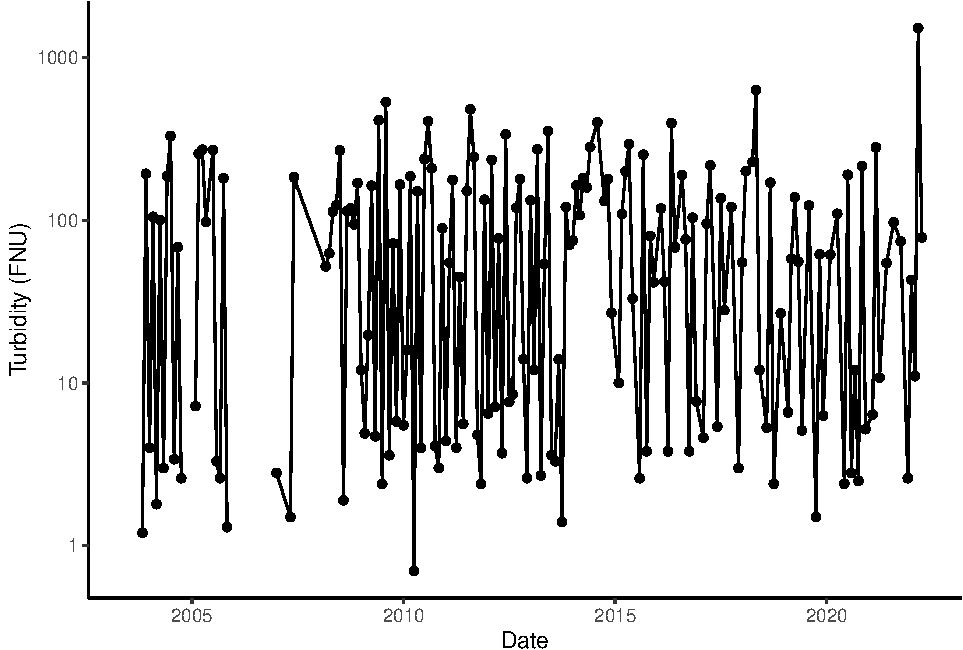
\includegraphics{Project_Template_files/figure-latex/Turbidity over time-1} \hfill{}

\caption{Turbidity of the North East Branch over time.}\label{fig:Turbidity over time}
\end{figure}

\newpage

Temperature was plotted to visualize any trends over time (Figure 2).
There are no obvious trends in temperature over time and a summary of
the data show that there are no missing values in the dataset. However,
around 2006 and 2007, a high temperature is not observed like the rest
of the time period. The mean temperature over the full time period is
14.45 degrees C.

\begin{figure}

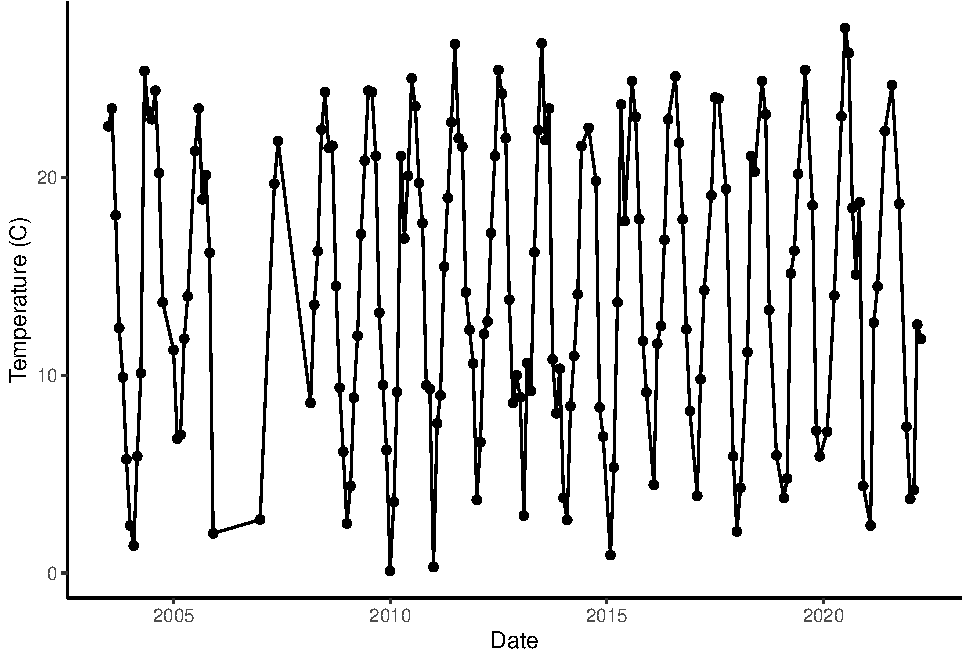
\includegraphics{Project_Template_files/figure-latex/Temperature over time-1} \hfill{}

\caption{Temperature of the North East Branch over time.}\label{fig:Temperature over time}
\end{figure}

\newpage

Specific conductance was plotted over time to visualize any major trends
in ionic concentration over time (Figure 3). The plot shows eight major
peaks in specific conductance from 2003 through 2022, with the highest
peak in 2021. A summary of the data show that the mean specific
conductance is 390.8 uS/cm and the maximum is 4640.0 uS/cm, which is an
order of magnitude larger. There are no missing values for specific
conductance in this dataset.

\begin{figure}

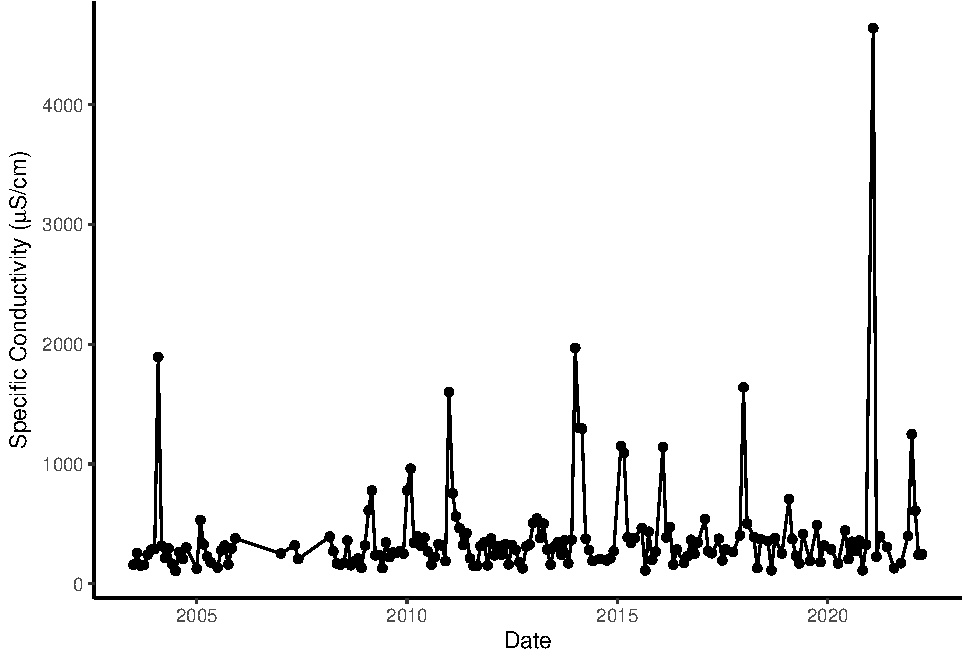
\includegraphics{Project_Template_files/figure-latex/Specific conductivity over time-1} \hfill{}

\caption{Specific conductivity of the North East Branch over time.}\label{fig:Specific conductivity over time}
\end{figure}

\newpage

Dissolved oxygen was plotted to visualize any major trends over time
(Figure 4). It appears that dissolved oxygen concentrations may be less
variable in recent years, but it is difficult to tell in the plot. A
summary of the data show that the average dissolved oxygen concentration
is 10.400 mg/L and that there is one missing value for dissolved oxygen
in this dataset.

\begin{figure}

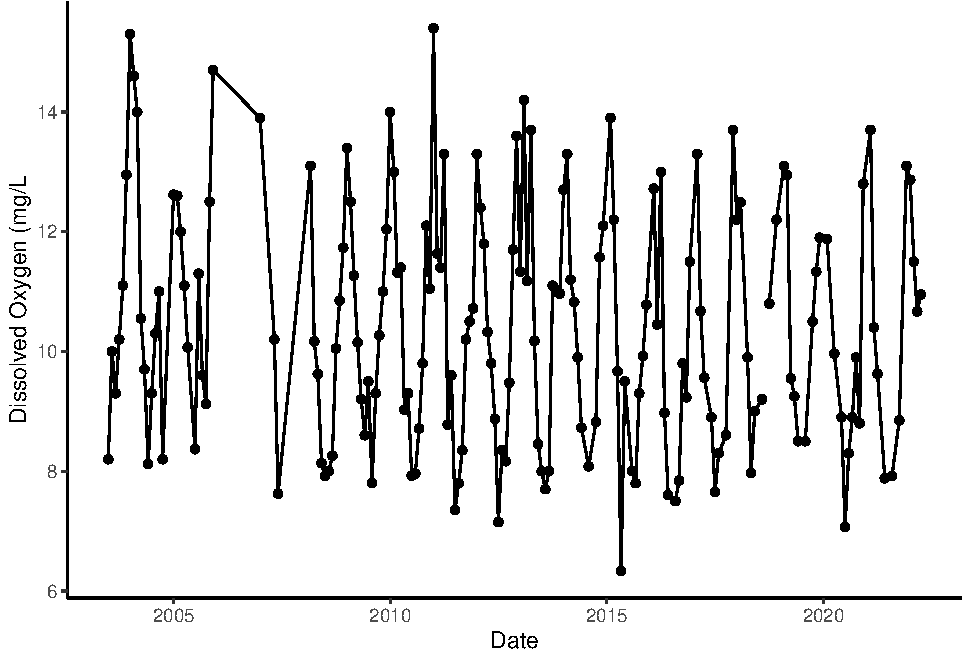
\includegraphics{Project_Template_files/figure-latex/Dissolved oxygen over time-1} \hfill{}

\caption{Dissolved oxygen concentration of the North East Branch over time.}\label{fig:Dissolved oxygen over time}
\end{figure}

\newpage

\hypertarget{analysis}{%
\section{Analysis}\label{analysis}}

\hypertarget{question-how-has-water-quality-changed}{%
\subsection{Question: How has water quality
changed?}\label{question-how-has-water-quality-changed}}

\hypertarget{turbidity}{%
\subsubsection{Turbidity}\label{turbidity}}

Time series analyses were conducted on turbidity for the time period
before the implementation of the Anacostia Watershed Restoration Plan
(2003 to 2009) (Figure 5) and after its implementation (2010-2022)
(Figure 6). A seasonal Mann-Kendall's test was conducted on both time
periods to test for stationarity. Both time periods display stationarity
and are neither significantly increasing or decreasing over time with
p-values greater that 0.05 (Table 2). While these data are not
statistically significant, it is worthwhile to consider the sign of the
tau values. Turbidity prior to the Plan's implementation was generally
increasing, while it is generally decreasing post-implementation. This
suggests that over a longer time period, stormwater control projects
could potentially reduce turbidity significantly.

\begin{figure}

{\centering 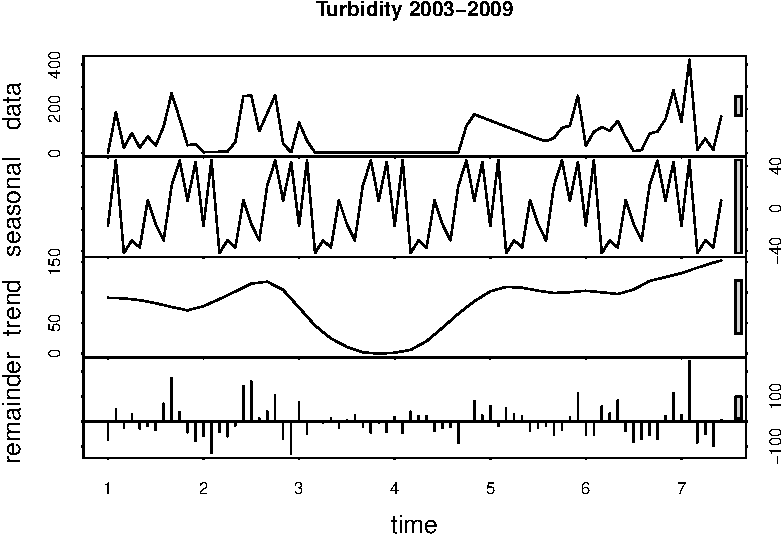
\includegraphics{Project_Template_files/figure-latex/Plot of Early Turbidity Time Series Decomposition-1} 

}

\caption{Time series decomposition of turbidity from 2003 to 2009.}\label{fig:Plot of Early Turbidity Time Series Decomposition}
\end{figure}

\begin{verbatim}
## NULL
\end{verbatim}

\begin{figure}

{\centering 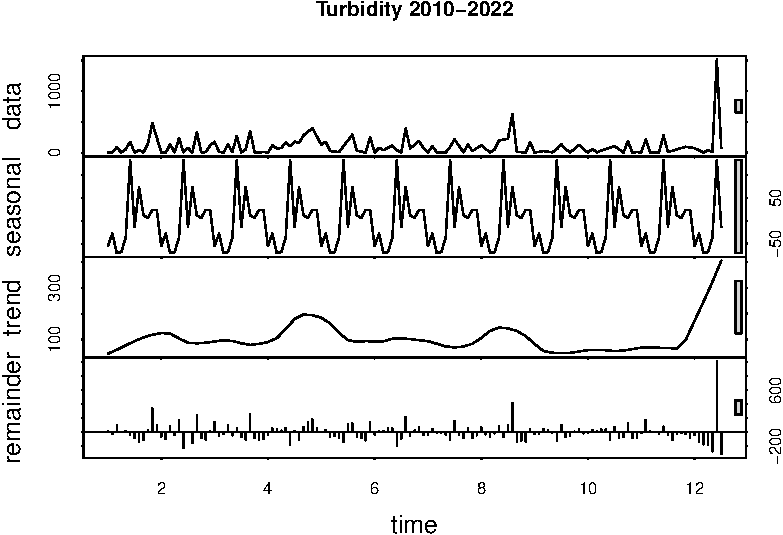
\includegraphics{Project_Template_files/figure-latex/Plot of Late Turbidity Time Series Decomposition-1} 

}

\caption{Time series decomposition of turbidity from 2010 to 2022.}\label{fig:Plot of Late Turbidity Time Series Decomposition}
\end{figure}

\begin{verbatim}
## NULL
\end{verbatim}

\newpage

\begin{figure}

{\centering 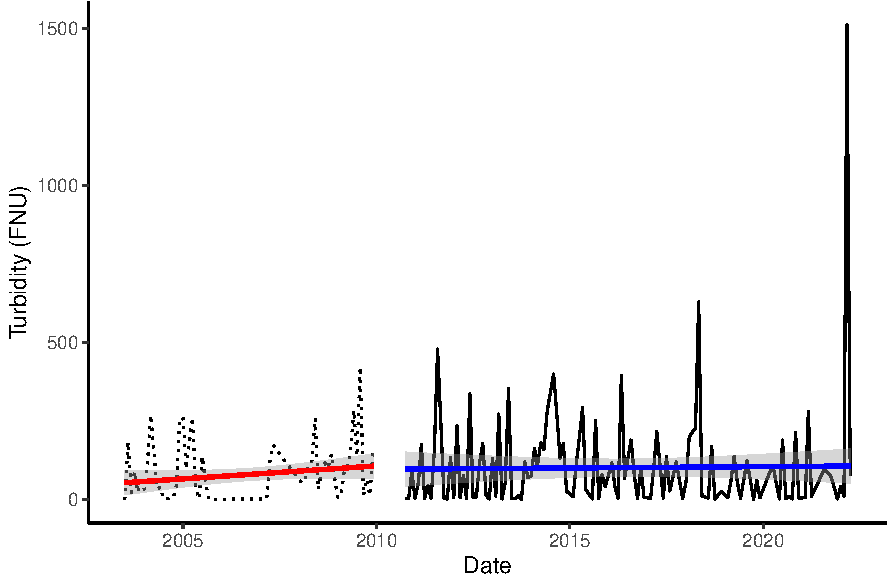
\includegraphics{Project_Template_files/figure-latex/Plot of Turbidity over time with LMs-1} 

}

\caption{Plot of turbidity over time with linear models from 2003 to 2009 and 2010 to 2022.}\label{fig:Plot of Turbidity over time with LMs}
\end{figure}

\newpage

\hypertarget{temperature}{%
\subsubsection{Temperature}\label{temperature}}

Time series analyses were conducted on temperature for the time period
before the implementation of the Anacostia Watershed Restoration Plan
(2003 to 2009) (Figure 7) and after its implementation (2010-2022)
(Figure 8). A seasonal Mann-Kendall's test was conducted on both time
periods to test for stationarity. Both time periods display stationarity
and are neither significantly increasing or decreasing over time with
p-values greater that 0.05 (Table 2). The Anacostia Watershed
Restoration Plan did not significanlty affect temperature in the
Northeast Branch.

\begin{figure}

{\centering 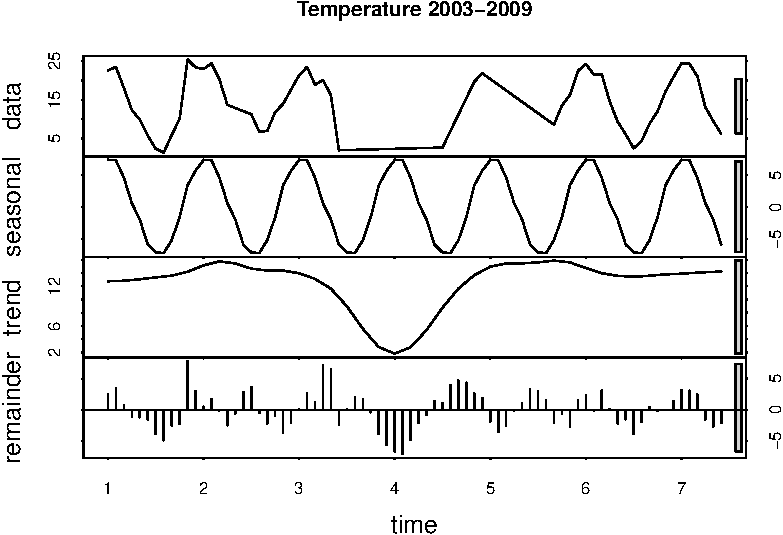
\includegraphics{Project_Template_files/figure-latex/Plot of Early Temperature Time Series Decomposition-1} 

}

\caption{Time series decomposition of temperature from 2003 to 2009.}\label{fig:Plot of Early Temperature Time Series Decomposition}
\end{figure}

\begin{figure}

{\centering 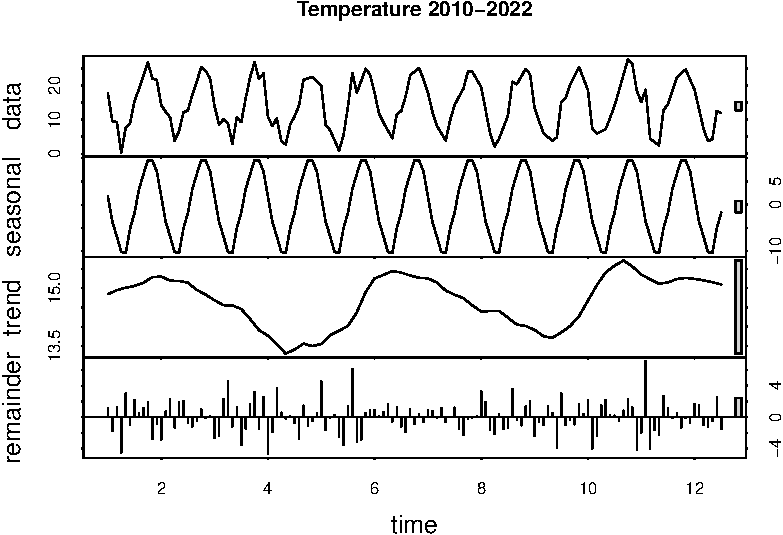
\includegraphics{Project_Template_files/figure-latex/Plot of Late Temperature Time Series Decomposition-1} 

}

\caption{Time series decomposition of temperature from 2010 to 2022.}\label{fig:Plot of Late Temperature Time Series Decomposition}
\end{figure}

\newpage

\begin{figure}

{\centering 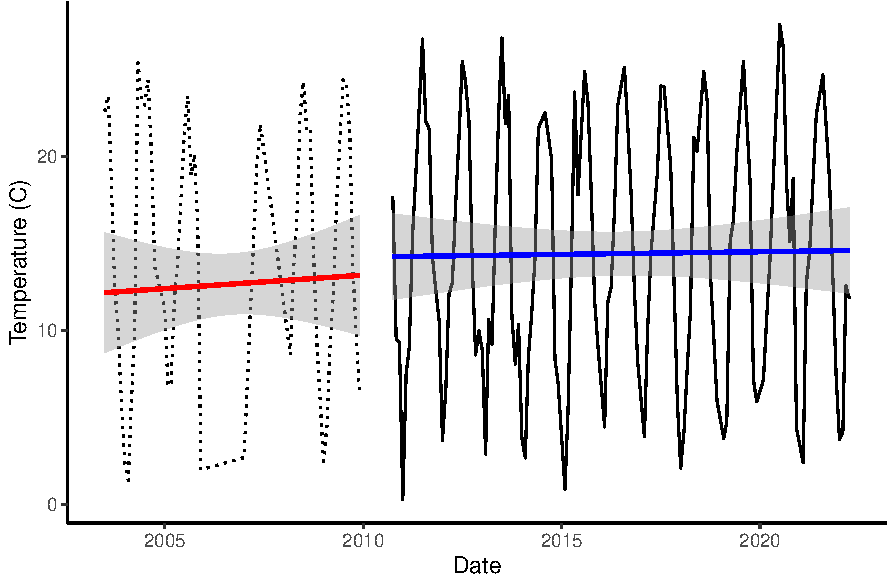
\includegraphics{Project_Template_files/figure-latex/Plot of Temperature over time with LMs-1} 

}

\caption{Plot of temperature over time with linear models from 2003 to 2009 and 2010 to 2022.}\label{fig:Plot of Temperature over time with LMs}
\end{figure}

\newpage

\hypertarget{specific-conductivity}{%
\subsubsection{Specific Conductivity}\label{specific-conductivity}}

Time series analyses were conducted on specific conductivity for the
time period before the implementation of the Anacostia Watershed
Restoration Plan (2003 to 2009) (Figure 9) and after its implementation
(2010-2022) (Figure 10). A seasonal Mann-Kendall's test was conducted on
both time periods to test for stationarity. Both time periods display
stationarity and are neither significantly increasing or decreasing over
time with p-values greater that 0.05 (Table 2). While these data are not
statistically significant, it is worthwhile to consider the sign of the
tau values. Specific conductivity prior to the Plan's implementation was
generally increasing, while it is generally decreasing
post-implementation. This suggests that over a longer time period,
stormwater control projects could potentially reduce specific
conductivity and the concentration of pollutants significantly.

\begin{figure}

{\centering 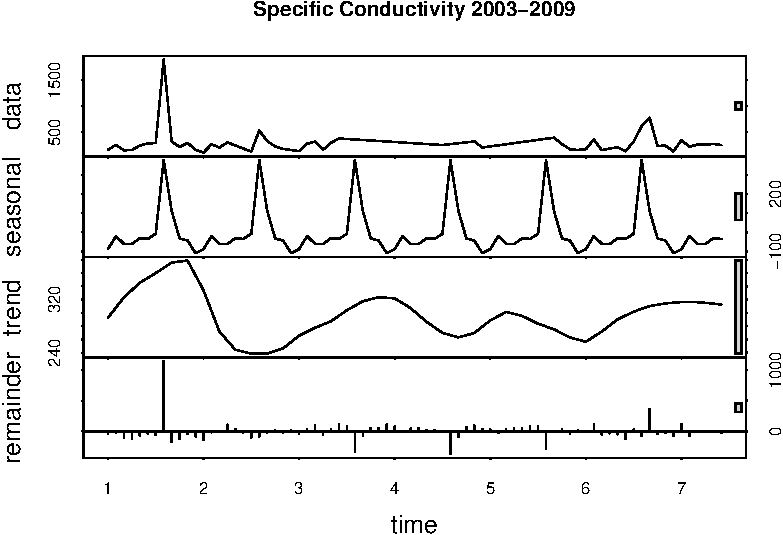
\includegraphics{Project_Template_files/figure-latex/Plot of Early Specific Conductivity Time Series Decomposition-1} 

}

\caption{Time series decomposition of specific conductivity from 2003 to 2009.}\label{fig:Plot of Early Specific Conductivity Time Series Decomposition}
\end{figure}

\begin{figure}

{\centering 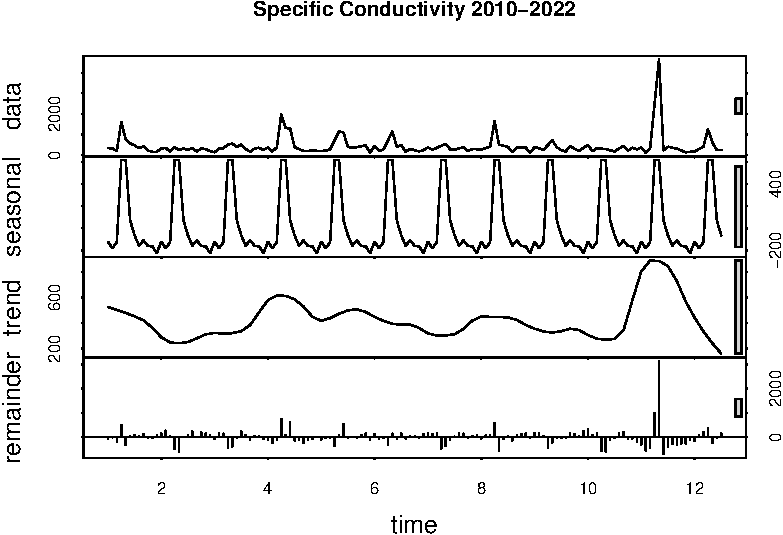
\includegraphics{Project_Template_files/figure-latex/Plot of Late Specific Conductivity Time Series Decomposition-1} 

}

\caption{Time series decomposition of specific conductivity from 2010 to 2022.}\label{fig:Plot of Late Specific Conductivity Time Series Decomposition}
\end{figure}

\newpage

\begin{figure}

{\centering 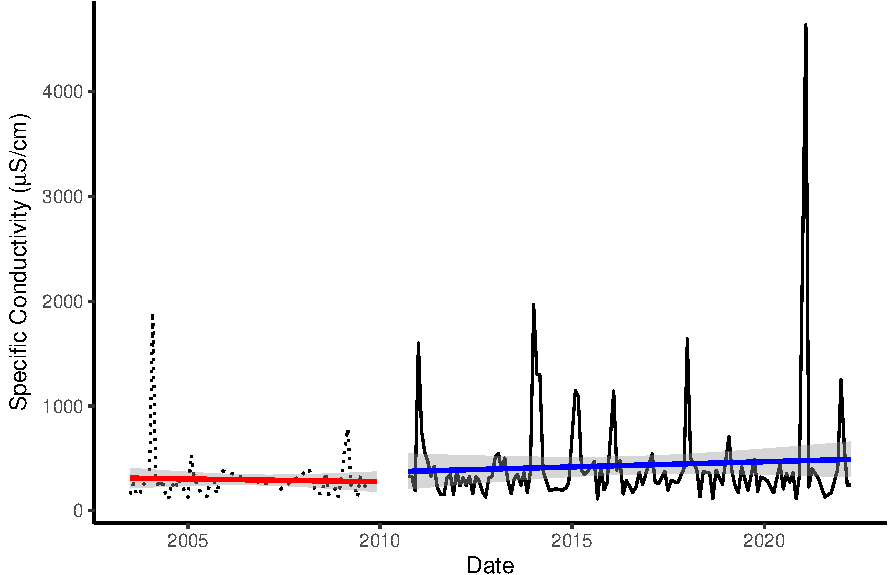
\includegraphics{Project_Template_files/figure-latex/Plot of Specific Conductance over time with LMs-1} 

}

\caption{Plot of specific conductivity over time with linear models from 2003 to 2009 and 2010 to 2022.}\label{fig:Plot of Specific Conductance over time with LMs}
\end{figure}

\newpage

\hypertarget{dissolved-oxygen}{%
\subsubsection{Dissolved Oxygen}\label{dissolved-oxygen}}

Time series analyses were conducted on dissolved oxygen for the time
period before the implementation of the Anacostia Watershed Restoration
Plan (2003 to 2009) (Figure 11) and after its implementation (2010-2022)
(Figure 12). A seasonal Mann-Kendall's test was conducted on both time
periods to test for stationarity. Both time periods display stationarity
and are neither significantly increasing or decreasing over time with
p-values greater that 0.05 (Table 2). The Anacostia Watershed
Restoration Plan did not significanlty affect dissolved oxygen in the
Northeast Branch.

\begin{figure}

{\centering 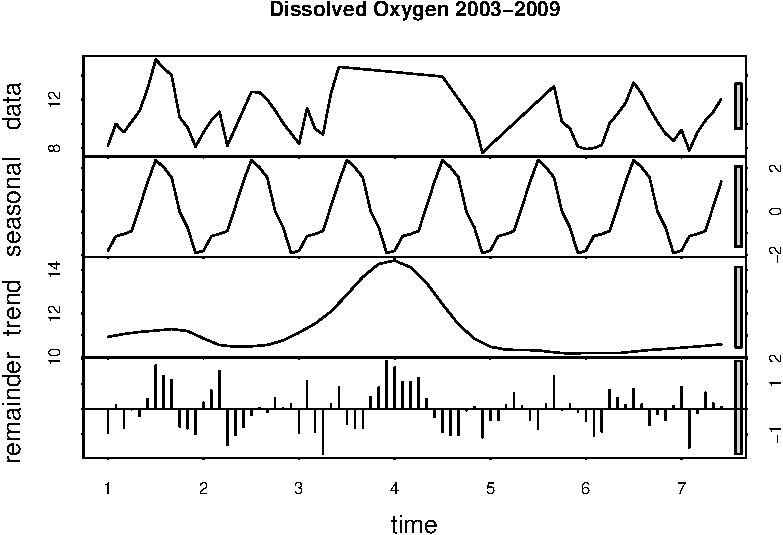
\includegraphics{Project_Template_files/figure-latex/Plot of Early Dissolved Oxygen Time Series Decomposition-1} 

}

\caption{Time series decomposition of dissolved oxygen from 2003 to 2009.}\label{fig:Plot of Early Dissolved Oxygen Time Series Decomposition}
\end{figure}

\begin{figure}

{\centering 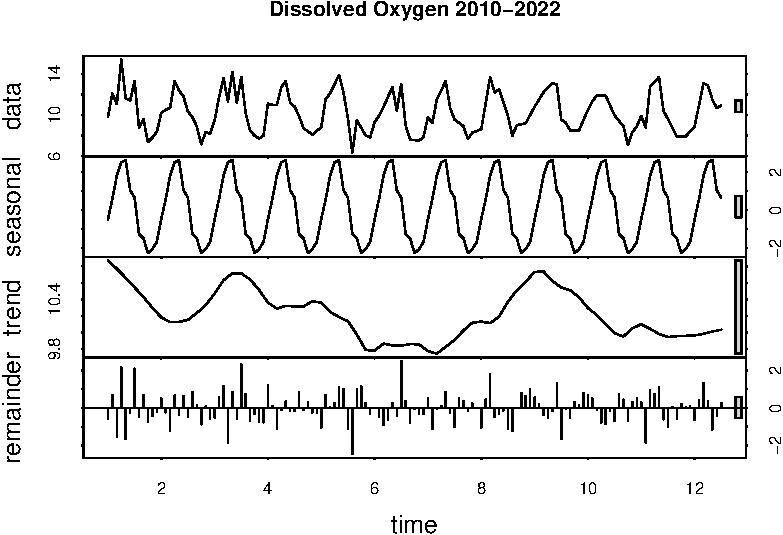
\includegraphics{Project_Template_files/figure-latex/Plot of Late Dissolved Oxygen Time Series Decomposition-1} 

}

\caption{Time series decomposition of dissolved oxygen from 2010 to 2022.}\label{fig:Plot of Late Dissolved Oxygen Time Series Decomposition}
\end{figure}

\newpage

\begin{figure}

{\centering 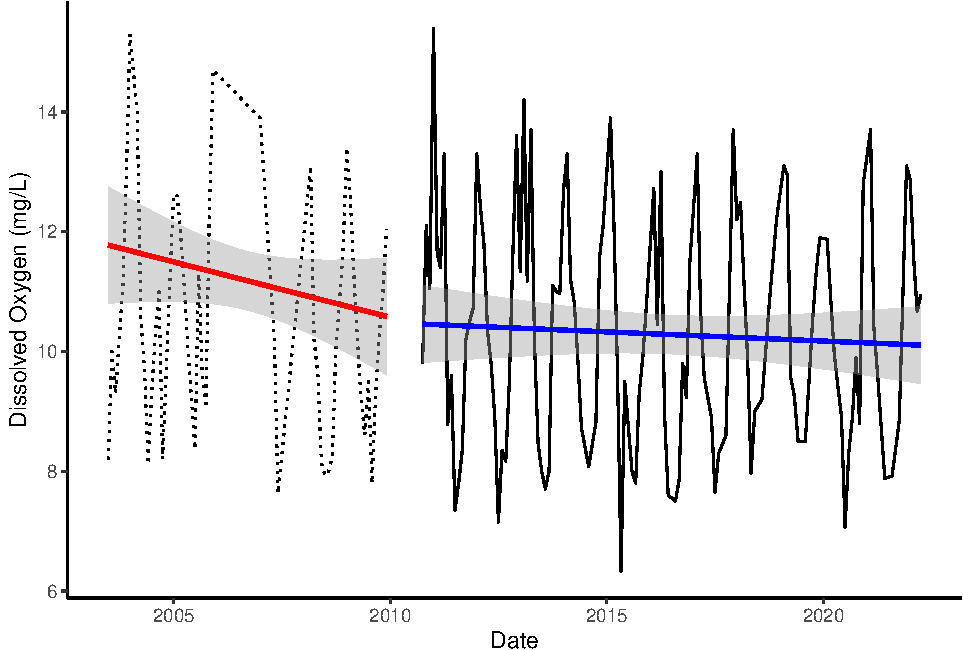
\includegraphics{Project_Template_files/figure-latex/Plot of Dissolved Oxygen over time with LMs-1} 

}

\caption{Plot of dissolved oxygen over time with linear models from 2003 to 2009 and 2010 to 2022.}\label{fig:Plot of Dissolved Oxygen over time with LMs}
\end{figure}

\newpage

\textbf{Table 2:} Summary of results from stationarity tests.

\begin{longtable}[]{@{}llll@{}}
\toprule
Parameter & Time Period & tau & p-value \\
\midrule
\endhead
Turbidity & Before & 0.13 & 0.17993 \\
. & After & -0.0992 & 0.12894 \\
Temperature & Before & 0.144 & 0.13719 \\
. & After & 0.0245 & 0.70806 \\
Specific Conductivity & Before & 0.0926 & 0.33815 \\
. & After & -0.0258 & 0.69284 \\
Dissolved Oxygen & Before & -0.181 & 0.061497 \\
. & After & -0.0626 & 0.33838 \\
\bottomrule
\end{longtable}

\newpage

\hypertarget{summary-and-conclusions}{%
\section{Summary and Conclusions}\label{summary-and-conclusions}}

Time series analyses and linear models conducted on turbidity,
temperature, specific conductivity, and dissolved oxygen on the time
periods both before and after the implementation of the Anacostia
Watershed Restoration Plan in 2010 were not significant. Therefore, no
concrete conclusions can be drawn from this analysis. However, we can
speculate that turbidity and specific conductivity may decrease in the
future given longer datasets.

\newpage

\hypertarget{references}{%
\section{References}\label{references}}

Metropolitan Washington Council of Governments. (2010, April 19).
Officials Release Landmark Anacostia Watershed Plan. Retrieved from
Newsroom:
\url{https://www.mwcog.org/about-us/newsroom/2010/04/19/officials-release-landmark-anacostia-watershed-plan-anacostia-restoration-water-quality/}

US Army Corps of Engineers (USACE). (2022, April 26). Anacostia
Watershed Restoration. Retrieved from Baltimore District Website:
\url{https://www.nab.usace.army.mil/Missions/Environmental/Anacostia-Watershed-Restoration/}

\end{document}
